
\begin{frame}[fragile]
%--------------------------------------------------  
 \secframetitle{\ssScaling}
\framesubtitle{Hydro, dark matterparticles, gravity: ``Cosmology (unigrid)'' problem}
%--------------------------------------------------

\textbf{We tested scaling of more recent support for cosmology}

\begin{minipage}{1.5in}
  \vspace{0.2in}
  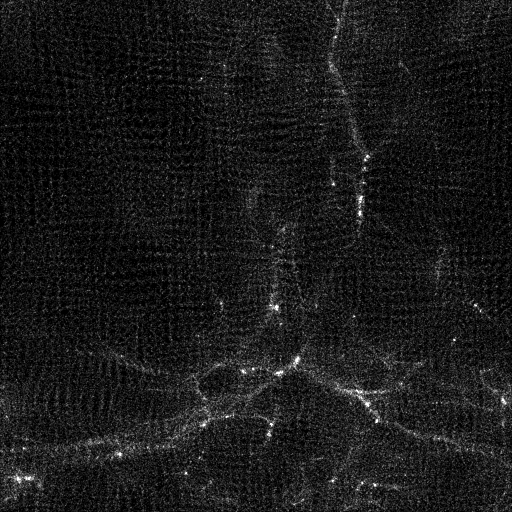
\includegraphics[width=1.5in]{Images/Cosmo/dark-20-normal.png} \\
%\centerline{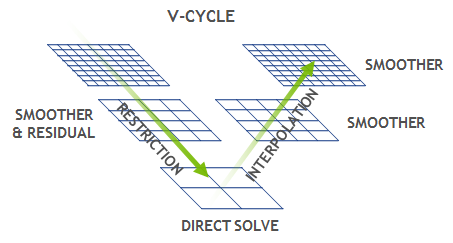
\includegraphics[width=1.5in]{hpgmg_v_cycle.png}}
\end{minipage} \
\begin{minipage}{2.75in}
  \vspace {0.2in}
  \begin{itemize}
  \item PPM hydrodynamics
  \item ``dark matter'' particles
  \item PM gravity method
  \item multigrid solver---(``unigrid'' only)
   \item tested up to $128K$ fp-cores
%  \item have since implemented AMR solver
%    \begin{itemize}
%      \item Dan Reynolds ``HG'' algorithm
%    \item preconditioned Krylov solver
%    \item multigrid-based preconditioner
%    \item effective up to $\approx 5$ levels
%    \end{itemize}
  \end{itemize}
\end{minipage}
\end{frame}
